\documentclass[a4paper,10pt]{scrreprt}
	\usepackage{sty/package}
	\usepackage{sty/document}
	\usepackage{sty/math}
	\usepackage{chngcntr}
	\usepackage{mathtools}
	\usepackage{algorithm2e}
	\usepackage{enumitem}
	\usepackage{graphicx}
	\usetikzlibrary{positioning}
	\usetikzlibrary{arrows}

	\lstset{
	basicstyle=\ttfamily,
	mathescape
	}
	\setlength\parindent{0pt}
	
	\pagestyle{fancy}
	\fancyhead[R]{Netzwerkalgorithmen}
	
	\counterwithout{section}{chapter}
	\counterwithin{figure}{section}
	\setcounter{chapter}{1}
	
	\renewcommand{\labelitemi}{$-$}
	
	\renewcommand*{\algorithmcfname}{Algorithmus}
	\RestyleAlgo{boxed}
	\LinesNumbered
	\SetKwInOut{Input}{Eingabe}
	\SetKwInOut{Output}{Ausgabe}

\begin{document}
	\section{Graphen}
	\begin{definition}[Ungerichteter Graph]
		Ein \textbf{ungerichteter Graph} $G$ ist ein Tripel $(V, E, \Psi)$, für das
		\begin{enumerate}
			\item $V$ und $E$ endliche Mengen sind und
			\begin{itemize}
				\item $V$ ist die Knotenmenge
				\item $E$ ist die Kantenmenge
			\end{itemize}
			\item $\Psi$ eine Funktion mit
			\begin{equation*}
				\Psi : E \to \set{X \subseteq V \vert 1 \le \card{X} \le 2}
			\end{equation*}
			ist.\\
		\end{enumerate}
		\begin{itemize}
				\item Zwei Kanten $e, e'$ sind \textbf{parallel}, wenn $\Psi(e) = \Psi(e')$.
				\item Eine Kante $e$ ist eine \textbf{Schleife}, falls $\card{\Psi(e)} = 1$.
				\item Ein Graph ohne parallele Kanten und Schleifen heißt \textbf{einfach}. Man schreibt dann $G = (V, E)$ mit $E(G)$ der Kantenmenge von G.
				\begin{itemize}[label=$\hookrightarrow$]
					\item  In einem einfachen Graphen kann man $\set{v_i, v_j}$ für eine Kante $e_{i,j}$ zwischen $v_i$ und $v_j$ schreiben.
				\end{itemize}
				\item $\card{E}$ ist die Zahl der Kanten und $\card{V}$ die Zahl der Knoten von $G$.
				\begin{itemize}[label=$\hookrightarrow$]
					\item Oft verwendet man $n$ für $\card{V}$ und $m$ für $\card{E}$.
				\end{itemize}
			\end{itemize}
	\end{definition}
	\begin{definition}[Nachbarschaft in Graphen]
		Eine Kante $e = \set{v, w}$ in einem Graphen verbindet zwei Knoten $v$ und $w$. Der Knoten $v$ ist dann Nachbar von $w$, d.h. $v$ und $w$ sind \textbf{adjazent} (\dq benachbart\dq). Außerdem ist sowohl $v$ als auch $w$ \textbf{inzident} (\dq zusammentreffend mit\dq) zu $e$.
	\end{definition}
	\begin{definition}[Knotengrad]
		Der \textbf{Grad} eines Knotens $v$ ist die Anzahl der inzidenten Kanten und wird bezeichnet mit $deg(v)$ (auch $\delta(v)$).\\[5pt]
		Ein Knoten $v$ heißt \textbf{isoliert}, wenn $deg(v) = 0$.
	\end{definition}
	\begin{satz}
		Sei $G = (V, E)$ ein Graph. Dann gilt
		\begin{equation*}
			\sum_{v \in V} deg(v) = 2\card{E}.
		\end{equation*}
		D.h. die Summe über alle Knotengrade ist gleich 2-mal die Anzahl der Kanten.
	\end{satz}
	\begin{lemma}[Handshake-Lemma]
		In jedem Graphen ist die Anzahl der Knoten mit ungeradem Grad gerade.
	\end{lemma}
	\begin{definition}[Teilgraph]
		Ein Teilgraph $H = (V(H), E(H))$ eines Graphen $G =\\ (V(G), E(G))$ ist ein Graph mit
		\begin{eqnarray*}
			V(H) &\subseteq& V(G),\\
			E(H) &\subseteq& E(G).
		\end{eqnarray*}
		$H$ ist \textbf{aufspannend}, wenn $V(H) = V(G)$ gilt.
	\end{definition}
	\begin{definition}[Isomorph]
		Seien $G = (V(G), E(G))$ und $H = (V(H), E(H))$ zwei Graphen. Wenn es eine bijektive Abbildung $f : V(G) \to V(H)$ gibt, sodass $\set{v, w} \in E(G)$ gilt, genau dann, wenn $\set{f(v), f(w)} \in E(H)$ gilt, dann nennen wir die Graphen \textbf{äquivalent} (oder \textbf{isomorph}).
	\end{definition}
	
	\subsection{Datenstrukturen für Graphen}
	\begin{definition}[Adjazenzmatrix]
		Eine \textbf{Adjazenzmatrix} $A = (a_{vw})$ eines Graphen $G = (V, E)$ beschreibt, welche Knoten $v_i$ zu welchen Knoten $v_j$ adjazent sind ($v_i, v_j \in V$). Die Matrix hat die Dimension $n\times n$, wobei $n = \card{V}$.\\
		Es gilt $A\in \set{0, 1}^{n\times n}$ mit
		\begin{equation*}
			a_{vw} := \begin{cases*}
				1 \text{ für } \set{v,w} \in E\\
				0 \text{ sonst}
			\end{cases*}
		\end{equation*}
		Eine Adjazenzmatrix ist quadratisch und symmetrisch. Für einfache Graphen enthält die Diagonale ausschließlich Nullen.\\
	\end{definition}
	\begin{definition}[Inzidenzmatrix]
		Eine \textbf{Inzidenzmatrix} $A = (a_{ve})$ eines Graphen $G = (V, E)$ beschreibt, welche Knoten $v_i \in V$ zu welchen Kanten $e_j \in E$ inzident sind. Die Matrix hat die Dimension $n\times m$, wobei $n = \card{V}$ und $m = \card{E}$.\\
		Es gilt $A\in \set{0, 1}^{n\times m}$ mit
		\begin{equation*}
			a_{ve} := \begin{cases*}
			1 \text{ für } v \in e\\
			0 \text{ sonst}
			\end{cases*}
		\end{equation*}
		Für große Graphen enthält die Matrix tendenziell viele Nullen.
	\end{definition}
	\begin{definition}[Kantenliste]
		Eine \textbf{Kantenliste} eines Graphen $G = (V, E)$ ist eine Liste aus zweielementigen Knotenmengen $\set{v_i, v_j} \in E$, die eine Kante von $v_i$ zu $v_j$ beschreiben $(v_i, v_j \in V)$.\\ Die Kantenliste benötigt $\Theta(m~log(n))$ Speicherplatz und ist damit sparsamer als die Inzidenzmatrix (für $n \ge 8$).
	\end{definition}
	\begin{definition}[Adjazenzliste]
		Eine \textbf{Adjazenzliste} eines Graphen $G = (V, E)$ gibt zu jedem Knoten $v_i$ die benachbarten Knoten $v_j$ an $(v_i, v_j \in V)$.\\
		Das ist etwas praktischer als die Kantenliste, wenn man für Graphenalgorithmen direkten Zugriff auf die Nachbarn eines Knotens benötigt. Man muss nicht die Nachbarn erst mühsam aus einer Liste heraussuchen.\\
		Die Adjazenzliste benötigt $\Theta(n~log(n)+m~log(n))$ Speicherplatz. Im Allgemeinen sind Graphen mit vielen isolierten Knoten (ohne Kanten) uninteressant, d.h z.B. $m\ge \frac{n}{2}$ oder $m\ge n$ o.ä. Also wieder $\Theta(m~log(n))$.
	\end{definition}
	
	\subsection{Wege und Pfade}
	\begin{definition}[Kantenfolge]
		Eine \textbf{Kantenfolge} $W$ in einem Graphen $G = (V, E)$ ist eine Folge $v_1, e_1, v_2, e_2, v_3, ..., e_k, v_{k+1}$ mit $k \ge 0,~e_i = \set{v_i, v_{i+1}} \in E$
	\end{definition}
	\begin{definition}[Weg]
		Wiederholt sich keine Kante in einer Kantenfolge, dann spricht man von einem \textbf{Weg}. Ein \textbf{geschlossener Weg} (auch Tour) kehrt am Ende zum Startknoten zurück. Ein \textbf{Eulerweg} benutzt alle Kanten eines Graphen. Eine \textbf{Eulertour} kehrt außerdem zum Startknoten zurück.
	\end{definition}
	\begin{definition}[Pfad]
		Wiederholt sich kein Knoten in einer Kantenfolge, dann sprichtman von einem \textbf{Pfad}. Ein \textbf{Kreis} ist ein geschlossener Pfad, d.h. der Pfad kehrt zum Startknoten zurück. Ein \textbf{Hamiltonpfad} besucht alle Knoten eines Graphen. Ein \textbf{Hamiltonkreis} (auch Hamiltontour) kehrt außerdem zum Startknoten zurück.
	\end{definition}
	\begin{satz}
		Sei $G$ ein Graph mit Adjazenzmatrix $A$. Der Koeffizient $a_{vw}^{(m)}$ von $A^m$ gibt die Anzahl der Kantenfolgen der Länge $m$ von Knoten $v$ zu Knoten $w$ an. Insbesondere gilt $a_{vv}^{(2)} = deg(v)$.
	\end{satz}
	\begin{definition}[Zusammenhängend]
		Ein Graph $G$ heißt \textbf{zusammenhängend}, wenn es zwischen je zwei Knoten aus $G$ einen Weg gibt.\\[5pt]
		Ein maximaler zusammenhängender Teilgraph von $G$ heißt eine \textbf{(Zusammenhangs-) Komponente} von $G$.
	\end{definition}
	\begin{satz}[notwendiges Kriterium]
		Ein zusammenhängender Graph $G$ mit $n$ Knoten muss zumindest $n - 1$ Kanten haben.
	\end{satz}
	\begin{satz}[hinreichendes Kriterium]
		Ein Graph $G$ mit mehr als $\frac{(n-1)(n-2)}{2}$ Kanten ist zusammenhängend.
	\end{satz}
	\begin{problem}[Zusammenhang]~\\[5pt]
		\hspace*{10pt}\textbf{Gegeben: } Ein Graph $G = (V, E)$.\\[5pt]
		\hspace*{10pt}\textbf{Gesucht: } Ist $G$ zusammenhängend?
	\end{problem}
	\begin{algorithm}[H]
		\Input{Graph $G$}
		\Output{Ist $G$ zusammenhängend}\vspace*{5pt}
		Markiere einen beliebigen Startknoten.\\
		Für jeden im voherigen Schritt markierten Knoten: Markiere alle noch nicht markierten adjazente Knoten. Wurde kein neuer Knoten markiert, dann 3. Sonst wiederhole 2.\\
		Sind noch unmarkierte Knoten übrig \Return \dq $G$ ist nicht zusammenhängend\dq. Sonst \dq$G$ ist zusammenhängend\dq.
		\caption{Algorithmus zum Entscheiden ob ein Graph $G$ zusammenhängend ist. Laufzeit: $O(\card{E})$}
	\end{algorithm}
	\begin{satz}
		Ein Graph $G$ mit Adjazenzmatrix $A$ ist zusammenhängend, genau dann, wenn
		\begin{equation*}
			Z = I_n + A + A^2 + ... + A^{n-1} \text{ mit } z_{vw} \neq 0~ \forall v, w \in \set{1, ..., n}
		\end{equation*}
		existiert.
	\end{satz}

	\subsection{Eulerwege und Hamiltonpfade}
	\begin{problem}[Eulerweg]~\\[5pt]
		\hspace*{10pt}\textbf{Gegeben: } Ein Graph $G = (V, E)$.\\[5pt]
		\hspace*{10pt}\textbf{Gesucht: } Ein Eulerweg $W$ in $G$ -  oder ein Argument, dass kein Eulerweg existiert.
	\end{problem}
	\begin{satz}
		Ein Graph $G = (V, E)$ besitzt genau dann einen Eulerweg, wenn es höchstens zwei Knoten mit ungeradem Grad gibt.
	\end{satz}
	\begin{algorithm}
		\Input{Graph $G$}
		\Output{Ein Weg in $G$}\vspace*{5pt}
		Starte in einem Knoten $v_0$ \newline(wenn einer mit ungeradem Grad existiert, dort, sonst beliebig)\\
		$i \leftarrow 0$\\
		\While{es gibt eine zu $v_i$ inzidente Kante}
		{wähle eine zu $v_i$ inzidente, unbenutze Kante $\set{v_i, v_j}$\\
		laufe zum Nachbarknoten $v_j$\\
		lösche $\set{v_i, v_j}$ aus der Menge der unbenutzen Kanten\\
		$v_{i+1} \leftarrow v_j$\\
		$i \leftarrow i+1$
		}
		\caption{Algorithmus zum Finden eines Weges in einem Graphen}
	\end{algorithm}
	\begin{satz}
		Wenn der Algorithmus 2 stoppt, bleibt ein eulerscher Graph zurück, d.h. ein Graph mit lauter Knoten geraden Grades.
	\end{satz}
	\begin{korollar}~
		\begin{enumerate}
			\item Zwei geschlossene Wege mit einem gemeinsamen Knoten kann man in einen geschlossenen Weg verwandeln.
			\item Man kann aus allen Wegen einen Weg machen, wenn der Graph zusammenhängend ist, indem man immer wieder 1. anwendet.
		\end{enumerate}
	\end{korollar}
	\begin{algorithm}
		\Input{Zusammenhängender Graph $G$ mit höchstens 2 ungeraden Knoten}
		\Output{Ein Eulerweg, bzw. eine Eulertour in $G$}\vspace*{5pt}
		Starte in einem Knoten $v$ \newline(wenn einer mit ungeradem Grad existiert, dort, sonst beliebig)\\
		verwende Algorithmus 2, um einen Weg $W$ von $v$ aus zu bestimmen\\
		\While{es existieren unbenutzte Kanten}
		{wähle einen Knoten $w$ aus $W$ mit positivem Grad im Restgraphen\\
		verwende Algorithmus 2, um einen Weg $W'$ von $w$ aus zu bestimmen\\
		verschmelze $W$ und $W'$\\
		}
		\caption{Algorithmus zum Finden eines Eulerweges oder einer Eulertour}
		\label{fig:Algorithmus}
	\end{algorithm}
	\begin{algorithm}[H]
		\Input{Zusammenhängender Graph $G$ mit höchstens 2 ungeraden Knoten}
		\Output{Ein Eulerweg, bzw. eine Eulertour in $G$}\vspace*{5pt}
		Starte in einem Knoten $v_0$ \newline(wenn einer mit ungeradem Grad existiert, dort, sonst beliebig)\\
		$i \leftarrow 0$\\
		\While{es gibt eine zu $v_i$ inzidente, unbenutzte Kante}
		{wähle eine dieser Kanten $\set{v_i, v_j}$, die den Restgraph zshgd. lässt\\
		laufe zum Nachbarknoten $v_j$\\
		markiere $\set{v_i, v_j}$ als benutzt\\
		$v_{i+1} \leftarrow v_j$\\
		$i \leftarrow i+1$
		}
		\caption{Algorithmus von Fleury zum Finden eines Eulerweges oder einer Eulertour}
	\end{algorithm}
	\begin{satz}[hinreichendes Kriterium]
		Wenn ein Graph mit $n$ Knoten mindestens $\frac{1}{2}(n-1)(n-2)+2$ Kanten hat, dann besitzt er einen Hamiltonkreis.
	\end{satz}

	\section{Minimale aufspannende Bäume}
	\begin{problem}[minimaler aufspannender Baum / kürzestes zsgd.es Netzwerk]~\\[5pt]
		\hspace*{10pt}\textbf{Gegeben: } Ein Graph $G = (V, E)$, Gewichtfunktion
		\begin{eqnarray*}
			c : E &\to& \reell_+\\
			e &\mapsto& c_e
		\end{eqnarray*}
		\hspace*{10pt}\textbf{Gesucht: } Eine Kantenmenge $F\subseteq E$ mit möglichst geringen Gesamtgewicht $\sum_{e \in F} c_e$, \hspace*{60pt}so dass in $T = (V, F)$ alle Knoten verbunden sind ODER entscheide, dass \hspace*{56pt} $G$ nicht zshgd. ist.
	\end{problem}\vspace*{10pt}
	\begin{enumerate}
		\item Welche Eigenschaften haben Lösungen?\\
		$\hookrightarrow$Struktur
		\item Wie findet man optimale Lösungen?
		\item Können wir algorithmische Grundideen verwenden, die auch in anderen Situationen funktionieren?
		\item Effizienz
	\end{enumerate}
	\begin{beobachtung*}
		Ein optimale Lösung für Problem 2.1 kann kein Kreis enthalten. (Beweisskizze: Entfernt man aus einem Kreis eine Kante bleibt der Rest immer noch verbunden).
	\end{beobachtung*}
	\begin{satz}
		Eine optimale Lösung für Problem 2.1 ist zusammenhängend und kreisfrei, also ein Baum.
	\end{satz}
	\begin{proof}
			Klar.
	\end{proof}
	Wir betrachten Eigenschaften von Bäumen. Wie viele Kanten hat ein Baum mit $n$ Knoten? Mit jeder eingefügten Kante nimmt die Zahl der Zhk. um 1 ab (mit jeder gelöschten um 1 zu).
	\begin{beobachtung*}
		Ein Baum mit $n$ Knoten hat $n-1$ Kanten. ABER: Nicht jeder Graph mit $n-1$ Kanten und $n$ Knoten ist ein Baum.
	\end{beobachtung*}
	\begin{definition}
		Für einen Graphen $G$ und $X,Y\subseteq V(G)$ ist
		\begin{eqnarray*}
			E(X,Y) &=& \set{\set{x,y}\in E(G)\vert x \in X\setminus Y,~y \in Y\setminus X}\\
			E^+(X,Y) &=& \set{(x,y)\in E(G)\vert x \in X\setminus Y,~y \in Y\setminus X}
		\end{eqnarray*}
		Für einen ungerichteten Graphen $G$ und $X \subseteq V(G)$
		\begin{equation*}
			\delta(X) = E(X, V(G)\setminus X)
		\end{equation*}
		Für einen gerichteten Graphen $G$ und $X\subseteq V(G)$
		\begin{eqnarray*}
			\delta^+(X) &=& E^+(X, V(G)\setminus X)\\
			\delta^-(X) &=& \delta^+(V(G)\setminus X)\\
			\delta(X) &=& \delta^+(X) \cup \delta^-(X)
		\end{eqnarray*}
	\end{definition}
	\begin{lemma}~
		\begin{enumerate}[a)]
			\item Ein ungerichteter Graph $G$ ist zusammenhängend $\Leftrightarrow \delta(X) \neq \emptyset~ \forall ~\emptyset \neq X \subset V(G)$.
			\item Sei $G$ ein gerichteter Graph und $r \in V(G)$. Dann gibt es einen Pfad von $r$ nach $v$ für jeden $v \in V(G) \Leftrightarrow \delta^+(X) \neq \emptyset~\forall~X\subset V(G)$ mit $r\in X$.
		\end{enumerate}
	\end{lemma}
	\begin{proof}
		
	\end{proof}
	
	\section{Kürzeste Wege}
\begin{problem}~\\[5pt]
	\hspace*{10pt}\textbf{Gegeben: }Gerichteter Graph $G$, Gewichte $c:A(G)\to \reell$, zwei ausgezeichnete \hspace*{60pt} Knoten $s,~t$.\\[5pt]
	\hspace*{10pt}\textbf{Gesucht: }$s$-$t$-Pfad minimalen Gesamtgewichts.
\end{problem}
Verschiedene Schwierigkeitsstufen
\begin{itemize}
	\item alle Kanten Einheitslänge $c(a)=1~ \forall a\in A(G)$.\\
	$\hookrightarrow$ (BFS) Suche nach Pfad mit minimaler Anzahl an Kanten.
	\item nicht negative Kantenlängen.\\
	$\hookrightarrow$ Dijkstra.
	\item ohne Kreise negativen Gesamtgewichts.
	\item allgemeine Kantengewichte.
\end{itemize}
\begin{definition*}[Konservativ]
	Sei $G$ ein Graph mit Gewichten $c:E(G)\to \reell$. Diese Kantengewichtsfunktion heißt \textbf{konservativ} wenn sie keine Kreise negativen Gesamtgewichts enthält.
\end{definition*}
\subsection{Kürzeste Wege von einer Quelle}
Algorithmen beruhen auf einer Beobachtung \dq Bellmans Prinzip\dq.
\begin{lemma}
	Sei $G$ ein Digraph mit konservativen Kantengewichten $c:A(G)\to \reell$, seinen $s$ und $w$ zwei Knoten. Ist $e=(v,w)$ die letzte Kante eines kürzesten Pfades $P$ von $s$ nach $w$, dann ist $P_{[s,v]}$ ($P$ ohne die Kante $e$) ein kürzester Pfad von $s$ nach $v$.
\end{lemma}
\begin{proof}
	Angenommen $Q$ ist ein kürzerer $s$-$v$-Pfad als $P_{[s,v]} \Rightarrow c(Q) + c(e) < c(P)$.
	\begin{itemize}
		\item Falls $Q$ $w$ nicht enthält $\Rightarrow Q + e$ ist kürzerer $s$-$w$-Pfad als $P$.
		\item Sonst gilt für $Q_{[s,w]}$:\\ $c(Q_{[s,w]}) = c(Q) + c(e) - c(Q_{[w,v]} + e) < c(P) - \underbrace{c(Q_{[w,v]} + e)}_{\mathclap{\text{ist ein Kreis und $c$ ist konservativ}}}) \le c(P)$\\ $\lightning$ $P$ ist kürzester $s$-$w$-Pfad.
	\end{itemize}
\end{proof}
Folgerungen:
\begin{itemize}
	\item Algorithmen bauen Wege schrittweise auf.
	\item Grund, dass meiste Algorithmen den kürzesten Weg von $s$ zu allen Knoten berechnen: Kürzesten $s$-$t$-Pfad berechnet $\Rightarrow$ auch kürzesten $s$-$v$-Pfad $\forall v\in P$ + wir wissen vorher nicht welche Knoten zu $P$ gehören.
\end{itemize}
Wir betrachten zunächst nicht-negative Kantengewichte. Sind diese auch ganzzahlig könnten wir auch BFS nutzen, indem wir Knoten durch Einheitskanten ersetzen.\\
Nachteil: Bläst Eingabe um exponentiellen Faktor auf. Statt
\begin{eqnarray*}
	&&\Theta(\underbrace{n~log(m)}_{\mathclap{\text{inzidente Kanten}}} + \underbrace{m~log(n)}_{Kanten} + \sum_{\mathclap{e \in E(G)}} log(c(e))) \text{ bekommen wir}\\
	&&\Theta(n'~log(m') + m'~log(n')) \text{ mit } m' = \sum_{\mathclap{e \in E(G)}} c(e),~n' = n + \sum_{\mathclap{e \in E(G)}} c(e) - 1
\end{eqnarray*}
Besser: Dijkstra.
\begin{definition}
	Sei $G$ ein Digraph mit $s, v \in V(G)$. Wir definieren
	\begin{itemize}
		\item $L(v) :=$ Länge eines kürzesten $s$-$v$-Pfades
		\item $p(v) :=$ Vorgänger von $v$ in einem kürzesten $s$-$v$-Pfad
	\end{itemize}
	($v$ nicht erreichbar: $L(v) = \infty,~p(v) = \text{NIL}$).
\end{definition}
\begin{algorithm}
	\Input{Digraph $G$, Gewichte $c:A(G)\to \reell_+$, Knoten $s\in V(G)$}
	\Output{Kürzeste Wege von $s$ zu allen $v\in V(G)$ und ihre Länge, genauer $L(v),~p(v)$}\vspace*{5pt}
	Setze $L(s) = 0$\\
	\hspace*{25pt}$L(v) = \infty~\forall v \in V(G)\setminus \set{s}$\\
	\hspace*{25pt}$R = \emptyset$\\
	Finde einen Knoten $v\in V(G)\setminus R$ mit $L(v) = \underset{\mathclap{w\in V(G)\setminus R}}{min}~L(w)$\\
	Setze $R = R \cup \set{v}$\\
	\For{$\forall w \in V(G)\setminus R$ mit $(v,w) \in A(G)$}{
		\If{$L(w)>L(v) + c((v,w))$}{
			Setze $L(w) = L(v) + c((v,w))$\\
			$p(w) = v$
		}
	}
	\If{$R\neq V(G)$}{\textbf{goto} 4}
	\caption{Dijkstras Algorithmus}
	\label{fig:Algorithmus}
\end{algorithm}
\begin{satz}
	Dijkstras Algorithmus ist korrekt. Die Laufzeit ist $O(n^2)$.
\end{satz}
\begin{proof}
	Wir zeigen, dass die folgenden Aussagen nach jeder Ausführung von 4. gelten
	\begin{enumerate}[a)]
		\item $\forall v\in R$ und $w\in V(G)\setminus R: L(v) \le L(w)$.
		\item $\forall v\in R: L(v)$ ist die Länge eines kürzesten $s$-$v$-Pfades in $G$. Wenn $L(v) < \infty$, dann existiert ein $s$-$v$-Pfad der Länge $L(v)$, dessen letzte Kante $(p(v), v)$ ist und dessen Knoten alle zu $R$ gehören.
		\item $\forall w\in V(G)\setminus R: L(w)$ ist die Länge eines kürzesten $s$-$w$-Pfades in $G[R\cup \set{w}]$. Wenn $L(w) \neq \infty$, dann $p(w)\in R$ und $L(w) = L(p(w)) + c((p(w),w))$.
	\end{enumerate}
	Die Aussagen gelten nach 1-3. Wir müssen zeigen, dass 5 und 6 die Gültigkeit von a), b) und c) aufrecht erhalten. Sei $v$ ein in 4 ausgewählter Knoten.\\
	zu a): Für jedes $x \in R,~y\in V(G)\setminus R$ gilt nach a) und der Wahl von $v$ in 4: $L(x) \le L(v) \le L(y) \Rightarrow$ a) gilt weiter nach 5 und 6.\\
	zu b): Zu zeigen: b) gilt nach 5 (dazu reicht: betrachte Knoten $v$). c) galt vor 5 $\to$ reicht zu zeigen, dass kein $s$-$v$-Pfad in $G$, der irgendein Knoten in $V(G)\setminus R$ enthält, kürzer ist als $L(v)$. Wir nehmen an es gebe einen $s$-$v$-Pfad $P$ in $G$, der einen knoten $w \in V(G)\setminus R$ enthält, der kürzer als $L(v)$ ist. Sei $w$ der erste Knoten außerhalb von $R$, wenn wir $P$ von $s$ nach $v$ durchlaufen. c) galt vor 5 $\Rightarrow L(w) \le c(P_{[s,w]})$. Kantengewichte nicht-negativ $\Rightarrow c(P_{[s,w]}) \le c(P) < L(v) \Rightarrow L(w) < L(v)~ \lightning$ Wahl von $v$ in 4.\\
	zu c): Wir zeigen, dass 5 und 6 c) aufrecht erhalten $\to$ wenn für $w$ (wir setzen $p(w) = v$ und $L(w) = L(v) + c((v,w))$) in 6 $\to$ existiert ein $s$-$v$-Pfad in $G[R \cup \set{w}]$ der Länge $L(v) + c((v,w))$ mit letzter Kante $(v,w)$ + wir wissen c) galt für $v$. Wir nehmen an, dass nach 5 und 6 ein $s$-$v$-Pfad $P$ in $G[R \cup \set{w}]$ existiert, der kürzer als $L(w)$ für ein $w\in V(G)\setminus R$ ist. $P$ muss $v$ enthalten - nur $w$ wurde hinzugefügt und sonst wäre c) schon vor 5 und 6 verletzt gewesen (wir wissen $L(w)$ wächst nicht). Sei $x$ der Nachbar von $w$ in $P$: $x \in R \overset{a)}{\Rightarrow} L(x) \le L(v) \overset{6}{\Rightarrow} L(w) \le L(x) + c((x,w)) \Rightarrow L(w) \le L(x) + c((x,w)) \le L(v) + c((x,w)) \le c(P) ~\lightning$ b) $\to$ $L(v)$ ist Länge eines kürzesten $s$-$v$-Pfades und $P$ enthält
	\begin{itemize}
		\item einen $s$-$v$-Pfad
		\item Kante $(x,w)$
	\end{itemize}
	Wir haben gezeigt:
	\begin{itemize}
		\item a), b) und c) gelten je in 4
		\item b) gilt insbesondere, wenn der Algorithmus terminiert\\
		$\hookrightarrow$ Ausgabe korrekt.
	\end{itemize}
	Laufzeit:
	\begin{itemize}
		\item $n$ Iterationen
		\item je $O(n)$
		\item[$\to$] $O(n^2)$
	\end{itemize}
\end{proof}
\begin{rem}
	\begin{itemize}
		\item $O(n^2)$ wieder bestmöglich für dichte Graphen.
		\item für \dq dünne\dq Graphen: Friedman und Tarjan (1987) haben mittels Fibonacci heaps die Laufzeit auf $O(n~log(n) + m)$ verbessert. Beste Laufzeit für nicht-negative Gewichte.
	\end{itemize}
\end{rem}
Jetzt: konservative Gewichte.
\begin{algorithm}
	\Input{Digraph $G$, konservative Gewichte $c:A(G)\to \reell$, Knoten $s\in V(G)$}
	\Output{Kürzeste Wege von $s$ zu allen $v\in V(G)$ und ihre Länge}\vspace*{5pt}
	Setze $L(s) = 0$\\
	\hspace*{25pt}$L(v) = \infty~\forall v \in V(G)\setminus \set{s}$\\
	\For{$i=1$ \textbf{to} $n-1$}{
		\For{jede Kante $(v,w)\in A(G)$}{
			\If{$L(w)>L(v) + c((v,w))$}{
				Setze $L(w) = L(v) + c((v,w))$\\
				$p(w) = v$
			}
		}
	}
	\caption{Moore-Bellman-Ford Algorithmus}
	\label{fig:Algorithmus}
\end{algorithm}
\begin{satz}
	Der Moore-Bellman-Ford Algorithmus ist korrekt und hat eine Laufzeit von $O(m\cdot n)$.
\end{satz}
\begin{proof}
	
\end{proof}
	\section{Netzwerkflüsse}
Flüsse in Graphen. Beispiele:
\begin{itemize}
	\item Wasser in Leitungssystemen
	\item Verkehr in Straßensystemen
	\item Passagiere in Transportsystemen
\end{itemize}
Eigenschaften:
\begin{itemize}
	\item pro Kante 2 Kenngrößen
	\begin{itemize}
		\item mögliche Flusskapazität
		\item tatsächlicher Fluss
	\end{itemize}
	\item \dq Flusserhaltung\dq : Bilanzierung der Flüsse an jedem Knoten (\dq fliest nicht mehr raus, als rein\dq)
\end{itemize}
\begin{definition}
	Gegeben: Digraph $G$ mit Kapazität $u: A(G) \to \reell_+$.
	\begin{enumerate}
		\item Ein \textbf{Fluss} ist eine Funktion $f: A(G) \to \reell_+$ mit $f(e) \le u(e)~\forall e\in A(G)$.
		\item An einem Knoten $v$ gilt \textbf{Flusserhaltung}, wenn \[\sum_{e\in \delta^-(v)} f(e) = \sum_{e\in \delta^+(v)} f(e).\]
		\item Eine \textbf{Zirkulation} ist ein Fluss für den an jedem Knoten Flusserhaltung gilt.
		\item Für ein Netzwerk $(G, u, s, t)$ ist ein Fluss ein $s$-$t$-Fluss, wenn Flusserhaltung an allen Knoten außer $s$ und $t$ gilt \[Wert(f) :=\sum_{e\in \delta^+(s)} f(e) - \sum_{e\in \delta^-(s)} f(e).\]
	\end{enumerate}
\end{definition}
\begin{problem}[Maximaler Fluss]~\\[5pt]
\hspace*{10pt}\textbf{Gegeben: }Netzwerk $(G, u, s, t)$.\\[5pt]
\hspace*{10pt}\textbf{Gesucht: }Ein $s$-$t$-Fluss mit maximalem Wert.
\end{problem}
Formulierung als LP (Lineares Programm):
\begin{eqnarray*}
	max~ F \text{ sodass} &&\sum_{e\in \delta^+(s)} f_e - \sum_{e\in \delta^-(s)} f_e = F,\\
	&&\sum_{e\in \delta^-(v)} f_e - \sum_{e\in \delta^+(v)} f_e = 0~\forall v\in V(G)\setminus \set{s,t},\\
	&&0\le f_e \le u_e~\forall e\in A(G).
\end{eqnarray*}
Also: Können wir effizient lösen (LP $\in$ P).\vspace*{5pt}\\
Ziel hier: \dq kombinatorische\dq Algorithmen.
\begin{beobachtung}
	Das Max Flow Problem hat immer eine optimale Lösung.
\end{beobachtung}
\begin{proof}~
	\begin{enumerate}
		\item LP ist beschränkt.
		\item Fluss mit $f\equiv 0$ ist immer zulässig.
	\end{enumerate}
\end{proof}
	\section{Matching}
\begin{definition}[Matching]~
	\begin{itemize}
		\item[i)] Ein \textbf{Matching} in einem Grap $G=(V,E)$ ist eine Menge paarweise disjunkter Kanten.
		\item[ii)] Ein Matching heißt \textbf{perfekt}, wenn jeder Knoten in $V(G)$ zu einer Matchingkante gehört.
		\item[iii)] Ein \textbf{Vertex Cover} ist eine Kantenüberdeckende Knotenmenge.
		\item[iv)] \textbf{Maximales Matching} in $G:$ $\mathcal{V}(G)$.
		\item[v)] \textbf{Minimales Vertex Cover} in $G:$ $\mathcal{T}(G)$.
	\end{itemize}
\end{definition}
\begin{figure}[ht]
	\begin{subfigure}[c]{0.5\textwidth}
		\begin{center}
			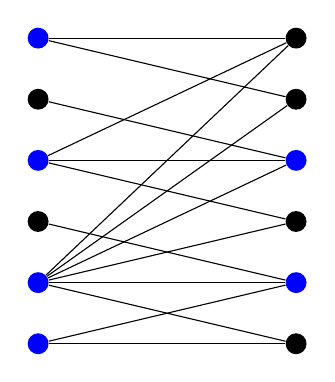
\begin{tikzpicture}
			\node[circle, fill, blue, scale = .8] (A) {};
			\node[circle, fill, black, scale = .8, below = 0.5cm of A] (B) {};
			\node[circle, fill, blue, scale = .8, below = 0.5cm of B] (C) {};
			\node[circle, fill, black, scale = .8, below = 0.5cm of C] (D) {};
			\node[circle, fill, blue, scale = .8, below = 0.5cm of D] (E) {};
			\node[circle, fill, blue, scale = .8, below = 0.5cm of E] (F) {};
			
			\node[circle, fill, black, scale = .8, right = 3cm of A] (H) {};
			\node[circle, fill, black, scale = .8, below = 0.5cm of H] (I) {};
			\node[circle, fill, blue, scale = .8, below = 0.5cm of I] (J) {};
			\node[circle, fill, black, scale = .8, below = 0.5cm of J] (K) {};
			\node[circle, fill, blue, scale = .8, below = 0.5cm of K] (L) {};
			\node[circle, fill, black, scale = .8, below = 0.5cm of L] (M) {};
			
			\path (A) edge (H);
			\path (A) edge (I);
			\path (B) edge (J);
			\path (C) edge (H);
			\path (C) edge (J);
			\path (C) edge (K);
			\path (D) edge (L);
			\path (E) edge (H);
			\path (E) edge (I);
			\path (E) edge (J);
			\path (E) edge (K);
			\path (E) edge (L);
			\path (E) edge (M);
			\path (F) edge (L);
			\path (F) edge (M);
			\end{tikzpicture}
		\end{center}
		\subcaption{Vertex Cover}
	\end{subfigure}
	\begin{subfigure}[c]{0.5\textwidth}
		\begin{center}
			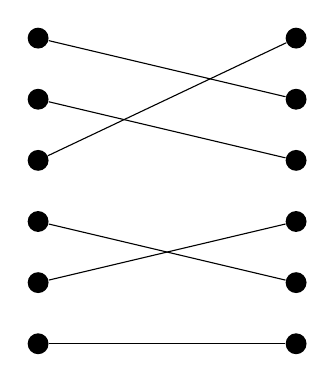
\begin{tikzpicture}[every loop/.style={}]
			\node[circle, fill, black, scale = .8] (A) {};
			\node[circle, fill, black, scale = .8, below = 0.5cm of A] (B) {};
			\node[circle, fill, black, scale = .8, below = 0.5cm of B] (C) {};
			\node[circle, fill, black, scale = .8, below = 0.5cm of C] (D) {};
			\node[circle, fill, black, scale = .8, below = 0.5cm of D] (E) {};
			\node[circle, fill, black, scale = .8, below = 0.5cm of E] (F) {};
			
			\node[circle, fill, black, scale = .8, right = 3cm of A] (H) {};
			\node[circle, fill, black, scale = .8, below = 0.5cm of H] (I) {};
			\node[circle, fill, black, scale = .8, below = 0.5cm of I] (J) {};
			\node[circle, fill, black, scale = .8, below = 0.5cm of J] (K) {};
			\node[circle, fill, black, scale = .8, below = 0.5cm of K] (L) {};
			\node[circle, fill, black, scale = .8, below = 0.5cm of L] (M) {};
			
			\path (A) edge (I);
			\path (B) edge (J);
			\path (C) edge (H);
			\path (D) edge (L);
			\path (E) edge (K);
			\path (F) edge (M);
			\end{tikzpicture}
		\end{center}
		\subcaption{Matching}
	\end{subfigure}
	\caption{Vertex Cover und Matching im bipartiten Graph}
\end{figure}
\begin{problem}[Kardinalitätsmatching/Max Matching]~\\[5pt]
	\hspace*{10pt}\textbf{Gegeben: }Ungerichteter Graph $G = (V,E)$.\\[5pt]
	\hspace*{10pt}\textbf{Gesucht: }Ein Matching $M$ größtmöglicher Kardinalität.
\end{problem}
\begin{problem}[Minimales Vertex Cover]~\\[5pt]
	\hspace*{10pt}\textbf{Gegeben: }Ungerichteter Graph $G = (V,E)$.\\[5pt]
	\hspace*{10pt}\textbf{Gesucht: }Ein Vertex Cover $C$ kleinstmöglicher Kardinalität.
\end{problem}
\begin{satz}
	Sei $G$ ein ungerichteter Graph. Es gilt max Matching $\le$ min Vertex Cover.
\end{satz}
\begin{figure}[ht]
	\begin{center}
		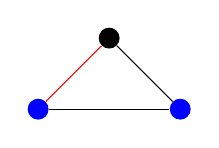
\begin{tikzpicture}
			\node[circle, fill, black, scale = .8] (A) {};
			\node[circle, fill, blue, scale = .8, below left = 1cm of A] (B) {};
			\node[circle, fill, blue, scale = .8, below right = 1cm of A] (C) {};
			
			\path (A) edge[red] (B);
			\path (A) edge (C);
			\path (B) edge (C);
		\end{tikzpicture}
		\end{center}
	\caption{max Matching $\le$ min Vertex Cover}
\end{figure}
\newpage
\begin{definition}[Bipartite Graphen]
	Ein Graph heißt \textbf{bipartit}, wenn sich die Knotenmenge so in zwei Mengen $A,B$ mit $V(G) = A \dot\cup B$ zerlegen lässt, dass jede Kante genau einen Knoten in $A$ und einen Knoten in $B$ enthält.
\end{definition}
\textit{Damit: Bipartite Graphen enthalten keine Kreise ungerader Länge. Für bipartite Graphen gibt es eine Beziehung zu Flussproblemen:}
\begin{center}
	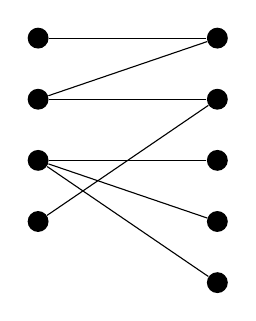
\begin{tikzpicture}
		\node[circle, fill, black, scale = .8] (A) {};
		\node[circle, fill, black, scale = .8, below = .5cm of A] (B) {};
		\node[circle, fill, black, scale = .8, below = .5cm of B] (C) {};
		\node[circle, fill, black, scale = .8, below = .5cm of C] (D) {};
		
		\node[circle, fill, black, scale = .8, right = 2cm of A] (E) {};
		\node[circle, fill, black, scale = .8, below = .5cm of E] (F) {};
		\node[circle, fill, black, scale = .8, below = .5cm of F] (G) {};
		\node[circle, fill, black, scale = .8, below = .5cm of G] (H) {};
		\node[circle, fill, black, scale = .8, below = .5cm of H] (I) {};
		
		\path (A) edge (E);
		\path (B) edge (E);
		\path (B) edge (F);
		\path (C) edge (G);
		\path (C) edge (H);
		\path (C) edge (I);
		\path (D) edge (F);
	\end{tikzpicture}
\end{center}
\textit{
\begin{itemize}
	\item füge 2 neue Knoten $s,t$ ein: Kanten von $s$ nach $v\in A$ und von $v\in B$ zu $t$.
	\item Kanten von $A$ nach $B$ richten.
	\item $u(e) = 1$ falls $s\in e$ oder $t\in e$, $u(e) = \infty$ sonst.
\end{itemize}
}
\begin{center}
	\begin{tikzpicture}
	\node[circle, fill, black, scale = .8, below left = 1.5cm of A, label = s] (S) {};
	\node[circle, fill, black, scale = .8] (A) {};
	\node[circle, fill, black, scale = .8, below = .5cm of A] (B) {};
	\node[circle, fill, black, scale = .8, below = .5cm of B] (C) {};
	\node[circle, fill, black, scale = .8, below = .5cm of C] (D) {};
	
	\node[circle, fill, black, scale = .8, below right = 1.5cm of E, label = t] (T) {};
	\node[circle, fill, black, scale = .8, right = 2cm of A] (E) {};
	\node[circle, fill, black, scale = .8, below = .5cm of E] (F) {};
	\node[circle, fill, black, scale = .8, below = .5cm of F] (G) {};
	\node[circle, fill, black, scale = .8, below = .5cm of G] (H) {};
	\node[circle, fill, black, scale = .8, below = .5cm of H] (I) {};
	
	\path (A) edge[->] node[above, scale = .8]{$\infty$} (E);
	\path (B) edge[->] node[above, scale = .8]{$\infty$} (E);
	\path (B) edge[->] node[above, scale = .8]{$\infty$} (F);
	\path (C) edge[->] node[above, scale = .8]{$\infty$} (G);
	\path (C) edge[->] node[above, scale = .8]{$\infty$} (H);
	\path (C) edge[->] node[above, scale = .8]{$\infty$} (I);
	\path (D) edge[->] node[above, scale = .8]{$\infty$} (F);
	\path (S) edge[->] node[above, scale = .8]{1} (A);
	\path (S) edge[->] node[above, scale = .8]{1} (B);
	\path (S) edge[->] node[above, scale = .8]{1} (C);
	\path (S) edge[->] node[above, scale = .8]{1} (D);
	\path (E) edge[->] node[above, scale = .8]{1} (T);
	\path (F) edge[->] node[above, scale = .8]{1} (T);
	\path (G) edge[->] node[above, scale = .8]{1} (T);
	\path (H) edge[->] node[above, scale = .8]{1} (T);
	\path (I) edge[->] node[above, scale = .8]{1} (T);
	\end{tikzpicture}
\end{center}
\textit{Aus gegebenen bipartiten Graph $G$ wird $(G',u,s,t)$.}
\begin{satz}
	Ein bipartites Matching maximaler Kardinalität in $G$ entspricht einem maximalen Fluss in $(G',u,s,t)$ und umgekehrt.
\end{satz}
\begin{proof}~
	\begin{itemize}
		\item Jedes Matching in $G$ lässt sich direkt auf einen Fluss in $G'$ abbilden, indem die Matchingkanten einen Fluss von jeweisl 1 erhalten und entsprechende Flüsse von $s$ und $t$ gewählt werden.
		\item Umgekehrt lässt sich jeder ganzzahliger Fluss (der auf jeder Kante den Wert 0 oder 1 hat) auf ein Matching in $G$ abbilden.
	\end{itemize}
	Da es immer ein ganzzahliges Optimum für das Flussproblem gibt, sind also insbesondere die Optimalwerte gleich.
\end{proof}
\begin{satz}
	In bipartiten Graphen gilt $\mathcal{V}(G) = \mathcal{T}(G)$.
\end{satz}
\begin{proof}
	$\mathcal{V}(G) = Max~Flow(G) = Min~Cut(G) \overset{!}{=} \mathcal{T}(G)$. Betrachte Min Cut $\delta^+(\set{s}\cup Q), Q \subseteq V$. Dieser Cut hat endliche Kapazität, d.h. es gibt keine Kante von $A \cap Q$ zu $B\setminus Q$.
	\begin{eqnarray*}
		A \cap Q & \text{ zu } & B \cap Q\\
		A \cap Q & \text{ zu } & B \setminus Q ~\lightning\\
		A \setminus Q & \text{ zu } & B \cap Q\\
		A \setminus Q & \text{ zu } & B \setminus Q
	\end{eqnarray*}
	Also ist jede Kante in $G$ inzident zu einem Knoten aus $C = (A\setminus Q)\cup (B \cap Q)$. D.h. $C$ ist ein Cover der Größe $\card{C} = \card{A\setminus Q} + \card{B\cap Q}$. Die Kapazität des Cuts ist ebenfalls $\card{C} = \card{A\setminus Q} + \card{B\cap Q}$ (nach Konstruktion) d.h. Min Cut = min Vertex Cover.
\end{proof}
\begin{satz}[Satz von Hall]
	Sei $G$ ein bipartiter Graph mit $V(G)=A\dot\cup B$. Dann hat $G$ ein $A$ überdeckendes Matching $\Leftrightarrow$ $\card{\underbrace{T(X)}_{\mathclap{\text{Menge der Nachbarn von } X}}} \ge \card{X}~\forall X\subseteq A$.
\end{satz}
\begin{proof}~
	\begin{itemize}
		\item Notwendigkeit ist klar.
		\item Um zu zeigen, dass auch hinreichend nehmen wir an $G$ hat kein $A$ überdeckendes Matching. $\mathcal{V}(G) \le \card{A} \overset{5.7}{\Rightarrow} \mathcal{T}(G) < \card{A}$. Sei $A' \subseteq A, B' \subseteq B$, so dass $A' \cup B'$ alle Kanten überdeckt und $\card{A' \cup B'} < \card{A} \Leftrightarrow \card{A'} + \card{B'} < \card{A}$ (da $A'$ und $B'$ disjunkt) $\Leftrightarrow \card{B'} < \card{A} - \card{A'}$. Es gilt $T(A\setminus A') \subseteq B'$ ( da $B'$ alle Kanten überdeckt, die nicht von $A'$ überdeckt werden) $\Rightarrow \card{T(A\setminus A')} \le \card{B'} < \card{A} - \card{A'} = \card{A\setminus A'}~\lightning$ Kontraposition der Hinrichtung gezeigt.
	\end{itemize}
\end{proof}
\begin{korollar}[Heiratssatz von Frobenius]
	Sei $G$ ein bipartiter Graph mit $V(G) = A\dot\cup B$. Dann hat $G$ ein perfektes Matching $\Leftrightarrow \card{A}=\card{B}$ und $\card{T(X)} \ge \card{X}~\forall X \subseteq A$.
\end{korollar}
\textit{Aus dem Beweis von Satz 5.7 folgt}
\begin{korollar}
	Das Kardinalitätsmatching-Problem kann in bipartiten Graphen in $O(n\cdot m)$ gelöst werden.
\end{korollar}
\begin{proof}
	Konstruktion von oben. Betrachte Ford-Fulkerson für das äquivalente Flussproblem
	\begin{itemize}
		\item Eine Augmentierung benötigt $O(m)$.
		\item Um einen maximalen $s$-$t$-Fluss (und damit ein maximales Matching) zu finden brauchen wir höchstens $n$ Augmentierungen $\Rightarrow$ $(O(m\cdot n))$.
	\end{itemize}
\end{proof}
\textit{Wie sehen Augmentierungen aus?\\
\hspace*{10pt}$\hookrightarrow$ Verbesserung von Matchings\\
Augmentierende Pfade in $(G',u,s,t)$ entsprechen alternierenden Pfaden in $G$.}
\begin{definition}
	Sei $G$ ein Graph (bipartit oder nicht), und sei $M$ ein beliebiges Matching in $G$. Ein Pfad $P$ ist ein \textbf{$M$-alternierender Pfad}, wenn $E(P)\setminus M$ ein Matching ist. Ein $M$-alternierender Pfad ist \textbf{$M$-augmentierend}, wenn seine Endpunkte nicht von $M$ überdeckt werden (er zwei nicht gematchte Knoten verbindet).
\end{definition}
\textit{Augmentierende Pfade müssen ungerade Länge haben.}
\begin{satz}[Berg, 1957]
	Sei $G$ ein Graph mit einem beliebigen Matching $M$. $M$ hat max Kardinalität $\Leftrightarrow$ es gibt keinen $M$-augmentierenden Pfad.
\end{satz}
\begin{proof}
	
\end{proof}

\end{document}
